\documentclass[../../几何与拓扑.tex]{subfiles}

\begin{document}
    
\chapter{单纯复形}

\section{有限单纯复形}

\begin{definition}
    称 \(  \mathbb{R} ^{n}  \)上的一个点集 \(  A =  \left\{  a_0,\cdots,a_{k}  \right\} ,k\ge 1 \)  是集合无关的,
    若 \(  \mathbb{R} ^{n}  \)上的向量集 \(  S =  \left\{ a_1-a_0,a_2-a_0,\cdots ,a_{k}-a_0 \right\}  \)是线性无关的.
    
    约定单点集是几何无关的.
\end{definition}


\begin{definition}
    设 \(  H  \)是 \(  \mathbb{R} ^{n}  \)的子集,其中 \(  n  \)充分大.称 \(  H  \)是 \(  \mathbb{R} ^{n}  \)的一个 \(  k  \)-维超平面,若存在 \(  \mathbb{R} ^{n}  \)的
     \(  k  \)维积空间 \(  V^{k}  \),以及向量 \(  x \in \mathbb{R} ^{n}  \),使得 \[
     H =  x+ V^{k}
     \]          
\end{definition}
你好呀


\begin{proposition}
    \(  \mathbb{R} ^{n}  \)上的点集 \(  A =  \left\{  a_0,\cdots,a_{k}  \right\}, k \ge 1  \) 是几何无关的,当且仅当 \(  A  \)上的点不落在同一个
    \(  \left( k-1 \right)   \)维超平面上.  
\end{proposition}

\begin{proof}

   若 \(  A  \)中的点几何无关,反过来假设  \(  A  \)中的点落在 \(  \left( k-1 \right)   \)维超平面 \(  H =  x+ V^{k-1}  \)上,则 \(  a_0-x,a_1-x  ,\cdots ,a_{k}-x  \in V^{k-1}\)    .
    此时 \[
    a_1-a_0,\cdots ,a_{k}-a_0 \in V^{k-1}
    \]矛盾,因为 \(  k-1  \)维线性空间中不可能有 \(  k  \)个线性无关的向量.
    
    
    另一方面,若 \(  \left\{ a_1-a_0,\cdots ,a_{k}-a_0 \right\}  \)线性相关, 则由这些向量张成的
    线性空间是 \(  k-1  \)维的,设为 \(  V^{k-1}  \),我们有 \[
    a_0,a_1,\cdots ,a_{k} \in \left( a_0+ V^{k-1} \right) 
    \]  落在同一个 \(  \left( k-1 \right)   \)维超平面上. 
    \hfill $\square$
\end{proof}

\begin{proposition}
     \(  \mathbb{R} ^{n}  \)的子集 \(  S =  \left\{  a_0,\cdots,a_{k}    \right\}  \)是几何无关,当且仅当 
     对于任意满足以下两条的 \(  t_{i}  \) \begin{enumerate}
        \item \(  \sum _{i= 0}^{k} t_{i}a_{i}= 0  \);
        \item \(  \sum _{i= 0}^{k} t_{i}= 0  \)  ;
     \end{enumerate}
     都有 \(  t_{i}= 0, i= 0, 1,\cdots,k   \) .
        
\end{proposition}


\begin{proposition}
    令 \(  A =  \left\{  a_0,\cdots,a_{k}    \right\}  \)是 \(  \mathbb{R} ^{n}  \)上几何无关的点集.则存在唯一过 \(  A  \)中所有点 的 \(  k  \)维超平面   .
\end{proposition}
\begin{proof}

    先说明存在性,设 \(  V^{k}  \)是 \(  \left\{ a_1-a_0,\cdots ,a_{k}-a_0 \right\}  \)张成的 \(  \mathbb{R} ^{n}  \)的线性子空间,则 \(  a_0+ V^{k}  \)是过 \(  A  \)中所有点的 \(  k  \)维超平面.      

    接下来说明唯一性,设有两个超平面过这些点,分别是 \[
    \begin{aligned}
    H^{k}& =  x + V^{k}\\ 
     F^{k}& =  y+ W^{k} 
    \end{aligned}
    \]

    通过做减法不难发现 \(  a_1-a_0,\cdots ,a_{k}-a_0  \)同时在   \(  V^{k}  \)和 \(  W^{k}  \)里,它们都是这些向量张成的空间,并且是唯一的,因此 \(  V^{k}= W^{k}  \).
    \(  H^{k}  \)和 \(  F^{k}  \)是同一个空间 的两个陪集,它们要么相等,要么无交,因此只能有 \(  H^{k} = F^{k}  \).       
    \hfill $\square$
\end{proof}


\begin{proposition}
    设 \(  A =  \left\{  a_0,\cdots,a_{k}    \right\}  \)是 \(  \mathbb{R} ^{n}  \)  上集合无关的点集.
    则通过 \(  A  \)的唯一的 \(  k  \)维超平面上的点,可以被唯一地写作 \[
    h =  \sum _{i= 0}^{k} t_{i}a_{i},\quad  \sum _{i= 0}^{k} t_{i} = 1
    \]  
\end{proposition}
\begin{remark}
    若 \(  \left\{  a_0,\cdots,a_{k}    \right\}  \)是 \(  \mathbb{R} ^{n}  \)上集合无关的点集,可以建立 \(  \mathbb{R} ^{k}  \)到过 \(  a_0,\cdots ,a_{k}  \)    的超平面 \(  H^{k}  \)间的一一对应.
    将\(  \mathbb{R} ^{k}  \)上坐标 \(  \left(  t_1,\cdots,t_k  \right)   \)上的点映为 \(  H^{k}  \)中的点 \(  \left( 1-\sum _{i= 1}^{k}t_{k} \right)   a_0+  \sum _{i= 1}^{k}t_{i}a_{i}\)     
\end{remark}


\begin{definition}{重心坐标}
    令 \(  A =  \left\{  a_0,\cdots,a_{k}    \right\}  \)是 \(  \mathbb{R} ^{n}  \)上集合无关的点集, \(  h  \)是过 \(   a_0,\cdots,a_{k}     \)的唯一 \(  k  \)维 超平面上的任意一点,
    将 \(  h  \)写作 \[
    h =  \sum _{i= 0}^{k} t_{i}a_{i},\quad \sum _{i= 0}^{k}t_{i}= 1
    \]   称 \(  t_0,t_1,\cdots ,t_{k}  \)维 \(  h  \)关于集合 \(  A  \)的重心坐标.     
\end{definition}


\begin{definition}
    设 \(  A =  \left\{  a_0,\cdots,a_{k}    \right\}  \)是 \(  \mathbb{R} ^{n}  \)上集合无关的点集, \(  n \ge k  \).则 由集合 \(  A  \)张成的 \textbf{k-维几何单形}或 \textbf{k-单形},记作 \(   \sigma ^{k}  \),
    为所有点 \(  x \in \mathbb{R} ^{n}  \)的构成的集合,其中 \[
    x =  \sum _{i= 0}^{k} t_{i}a_{i},\quad \sum_{i= 0}^{k} t_{i}= 1, \quad  t_{i}\ge 0,i= 0, 1,\cdots,k 
    \]      
\end{definition}

\begin{remark}
    \begin{enumerate}
        \item  \(   a_0,\cdots,a_{k}     \) 称为 \(   \sigma ^{k}  \)的顶点;
        \item 通常记 \(   \sigma ^{k} =  \left< a_0,\cdots,a_{k}    \right>  \).  
    \end{enumerate}
    
\end{remark}

\begin{definition}{凸包}
    设 \(  A  \)是 \(  \mathbb{R} ^{n}  \)的子集, \(  A  \)的凸包被定义为 包含了 \(  A  \)的最小的凸集,即 \[
    \bigcap_{ \Omega \text{是包含了}A\text{的一个凸集}} \Omega  
    \]    
\end{definition}
\hspace*{\fill} 

\begin{proposition}
    设 \(  A =  \left\{  a_0,\cdots,a_{k}    \right\}  \)是 \(  \mathbb{R} ^{n}  \)  上几何无关的点集.则 \(   \sigma ^{k} \left< a_0,\cdots,a_{k}    \right>  \)是 \(  A  \)的凸包.  
\end{proposition}

\begin{proof}
    设 \(  H^{k}  \)是过 \(  A  \)的唯一 \(  k  \)维超平面.   
    对于 \(  i= 0, 1,\cdots,k   \),定义 \[
    H_{i} =  \left\{ \left(   \alpha_0,\cdots,\alpha_{k-1}  \right) \in H^{k}:  \alpha _{i}\ge 0  \right\}
    \] 则 \(   \sigma ^{k} =  H_0\cap H_1\cap \cdots \cap H_{k}  \).由于凸集的交是凸集,只需证明每个 \(  H_{i}  \)是凸的, \(  i = 0, 1,\cdots,k   \).
    事实上,任取 \(  H_{i}  \)上两点 \(  x_1= \left(  \alpha _0 ,\cdots , \alpha_{k} \right),x_2 = \left( \beta _0 ,\cdots ,\beta _{k} \right)    \)  按重心坐标表示,我们有 \(   \alpha _{i}, \beta _{i}\ge 0  \).
    因此 \(  tx_1+ \left( 1-t \right)x_2, 0\le t\le 1   \)的重心坐标的第 \(  i  \)个分量为 \( t \alpha _{i}+\left( 1-t \right)\beta _{i}   \)       也 \(  \ge 0  \),这表明 
    \(  tx_1+ \left( 1-t \right)x_2 \in  H_{i}   \), \(  H_{i}  \)是凸的.上述讨论对于 \(  i= 0, 1,\cdots,k   \)均成立,因此 \(   \sigma ^{k}  \)是凸的.     


   现在任取\(  \mathbb{R} ^{n}  \)上包含了 \(  A  \)的凸集 \(  B  \),我们来证明 \( \sigma ^{k}\subseteq B  \).    对 \(  k  \)归纳, \(  k= 0  \)时结论平凡地成立, 假设 \(  k-1  \)时结论成立,则 \(  \left<a_1,\cdots ,a_{k} \right>  \)在 \(  B  \)里. 接下来尝试把
    \(   \sigma ^{k}  \)中任意一点写作 \(  ta_0+ \left( 1-t \right) x_1   \),其中 \(  x_1 \in  \left< a_1,\cdots,a_k  \right>  \). 设 \[
    x =  \sum _{i= 0}^{k} t_{i}a_{i},\quad  t_{i}\ge 0,\sum _{i= 0}^{k}t_{i}= 1
    \]  当 \(  t_0= 1  \)时,显然 \(  x \in  \sigma ^{k}  \),以下设 \(  t_0<1  \),则此时 \(  s: =  \sum _{i= 1}^{k}t_{k}>0  \)  
    定义 \[
    x_1: =  \sum _{i= 1}^{k} \frac{t_{i} }{ s} a_{k} 
    \]  则 \(  x_1 \in \left< a_1,\cdots,a_k  \right>  \),注意到 \[
    x =  t_0a_0+ sx_1,\quad  s + t_0= 1
    \] 由于 \(  B  \)是凸的,因此 \(  x \in B  \).这就说明了 \(   \sigma ^{k} \subseteq B  \).   
    \hfill $\square$
\end{proof}

\begin{definition}
    令 \(   \sigma ^{k} =  \left< a_0,\cdots,a_{k}  \right>  \) 是一个 \(  k  \)-单形.称 \(   \sigma ^{k}  \)上所有重心坐标都严格正的点的集合为 \textbf{开 \(  k  \)-单形 \(   \sigma ^{k}  \) }.  
\end{definition}


\begin{definition}
    令 \( \sigma ^{p}, \sigma ^{q}, p\le q\le n  \) 是 \(  \mathbb{R} ^{n}  \)上的两个单形.
    称 \(   \sigma ^{p}  \)是 \(   \sigma ^{q}  \)的一个 \textbf{\(  p  \)维面 },若 \(   \sigma ^{p}  \)的每个顶点也都是 \(   \sigma ^{q}  \)的顶点.
    
    若 \(   \sigma ^{p}  \)是 \(   \sigma ^{q}  \)的一个面,且 \(  p< q  \),则称 \(   \sigma ^{p}  \)是 \(   \sigma ^{q}  \)的一个真面.     
\end{definition}

\begin{remark}
   \begin{enumerate}
    \item  任意 \(  k  \)-单形 \(   \sigma ^{k}  \)都可以写作它的所有开单形的无交并(顶点自身也是开单形).  
    \item  设 \(  x  \)是 \(   \sigma ^{k}  \)上的一点,重心坐标为 \(  \left(  \alpha_0,\cdots,\alpha_{k}  \right)   \)  
            \begin{enumerate}
                \item 如果 \(  x  \)的坐标均大于零,则它在 \(   \sigma ^{k}  \)的内部;
                \item 如果 \(  x  \)的坐标有且仅有一个 \(  \alpha _{i}  \)等于零, 则它位于与 顶点\(  v_{i}  \) 相对的面的内部;
                \item 若 \(  x  \)的坐标有且仅有两个 \(  \alpha _{i},\alpha _{j}  \)等于零\(  \left( i\neq j \right)   \),则 \(  x  \)位于 \(   \sigma^{k}  \)的一个
                 \(  k-2  \)维面的内部.         
            \end{enumerate}
    
    \item 闭单形 \(  \left|  \sigma ^{k} \right|   \)上的所有点都可以通过唯一的非负重心坐标表示 \(  x =  \left(   \alpha_0,\cdots,\alpha_{k}  \right)   \), \(  \alpha _{i}\ge 0,\sum  \alpha _{i}= 1  \)   .
             
   \end{enumerate}
   
\end{remark}


\begin{proposition}
    投影映射 \(  p_{i}: \left|  \sigma ^{k} \right| \to [0,1]   \) , \(  p_{i}\left(  \alpha_0,\cdots,\alpha_{k}  \right)= \alpha _{k}   \) 是连续的.
\end{proposition}

\begin{proof}

    考虑 \(  \mathbb{R} ^{k+ 1}  \)的单位向量 \(   e_0,\cdots,e_{k}   \)存在 闭单形 \(  \left< v_0,\cdots,v_{k}  \right>  \)到闭单形 \(  \left< e_0,\cdots,e_{k}  \right>  \)的线性同胚\(  h  \), 
     \(  h\left( t_0v_0+ t_1v_1+ \cdots + t_{k}v_{k} \right) =  t_0e_0+ t_1e_1+ \cdots + t_{k}e_{k}   \).令 \(  q_{i} : \mathbb{R} ^{k+ 1}\to \mathbb{R}   \)是第 \(  i  \)个分量的标准投影,
     则 \(  q_{i}\circ h = p_{i}  \),因此 \(  p_{i}  \)连续.          

    \hfill $\square$
\end{proof}

\begin{definition}
    一个  \textbf{单纯复形}或者 \textbf{几何复形 } \(  K  \)由 \(  \mathbb{R} ^{m}  \)上
    的满足以下两条的有限多个单形构成,其中 \(  m  \)充分大 
    \begin{enumerate}
        \item 若 \(   \sigma  \in K  \),则 \(   \sigma  \)所有的面也在 \(  K  \)中;
        \item 若 \(   \sigma   \)和 \(  \tau   \)均在 \(  K  \)中,则要么 \(   \sigma \cap \tau = \varnothing  \),要么 \(   \sigma \cap \tau   \)是 \(   \sigma   \)和 \(  \tau   \)的公共面.          
    \end{enumerate}
     定义 \(  K  \)的 \textbf{维数},记作 \(  \operatorname{dim}\,K  \),当 \(  K= \varnothing  \)时为 \(  -1  \),当 \(  K  \)具有的最大维数的单形为 \(  k  \)-单形时为 \(  k  \).       
\end{definition}

\begin{remark}
    \begin{enumerate}
        \item 称第二个条件,为 \(   \sigma   \)和 \(  \tau   \)是良好连接的.  
    \end{enumerate}
    
\end{remark}



\begin{definition}
    设 \(   \sigma ^{k}  \)是 \(  k  \)-单形,全体 \(   \sigma ^{k}  \)   的面记作 \(  \operatorname{Cl}\,\left(  \sigma ^{k} \right)   \),称为 \(   \sigma ^{k}  \)的闭包.  
\end{definition}
\begin{example}
    \(   \sigma ^{2}= \left<a_0,a_1,a_2 \right>  \)的闭包是 \(  K   \) \[
    K =  \left\{ \left<a_0 \right>,\left<a_1 \right>,\left<a_2 \right>,\left<a_0,a_1 \right>,\left<a_0,a_2 \right> ,\left<a_1,a_2 \right>,\left<a_0,a_1,a_2 \right>\right\}
    \]  
\end{example}

\hspace*{\fill} 


\section{多面体和三角剖分}

在处理复杂的几何体时,最常用的一个方法是用“直”的几何体取近似代替它.对于那些可以被这样代替的几何体,也就是说
拓扑性质与某个“直”的几何体一样(同胚)的那些,我们叫他\textbf{多面体}.研究这一类几何体,只需要研究其对应的“直”的几何体,即单纯复形.

单纯复形的定义是一系列从具体的几何体抽象出来的结构,我们称对应的具体的几何体为它的几何载体.

为了研究单纯复形,自然地想要考虑不同单纯复形之间的关系,因此我们需要考虑保持单纯复形结构的映射,即单纯映射.
单纯映射可以看成是点对点、面对面、体对体的映射,这样的映射就已经能复刻出几何体的完全对应,它自然地给出一个从几何载体到几何载体的映射,我们称之为单纯映射诱导出的映射.
即我们找到单纯复形范畴到拓扑范畴的一个函子.




\begin{introduction}
    \item 单纯复形的几何载体、多面体
    \item 有界凸开集的同胚定理
    \item 抽象单纯复形
    \item 单纯映射及其在几何载体上的诱导
    \item 单纯复形的连通性
\end{introduction}

\begin{definition}
    令 \(  K  \)是一个单纯复形. 令 \(  \left| K \right| =  \bigcup_{ \sigma  \in K} \sigma     \)是 \(  K  \)的所有单形的并.
    对于某个 \(  n  \), \(  \left| K \right|   \)成为 \(  \mathbb{R} ^{n}  \)的一个子集,并且具有 \(  \mathbb{R} ^{n}  \)的子空间拓扑.此时称 \(  \left| K \right|   \)为 \(  K  \)的几何载体.
    若 \(  \mathbb{R} ^{n}  \)的一个子空间也是某个单纯复形的\textbf{几何载体},则该子空间也被称为是一个\textbf{直线多面体}.           
\end{definition}


\begin{definition}
    称拓扑空间 \(  X  \)为一个\textbf{多面体},若存在单纯复形 \(  K  \),使得 \(  \left| K \right|   \)与 \(  X  \)同胚.    
    此时, \(  X  \)被称为是可三角剖分的, \(  K  \)被称为是 \(  X  \)的三角剖分.   
\end{definition}

\hspace*{\fill} 


\begin{proposition}
    设 \(  U  \)是 \(  \mathbb{R} ^{n}  \)上的有界凸开集, \(  n\ge 1  \)  ,并且 \(   \omega  \in U  \),则
    \begin{enumerate}
        \item 每个从 \(   \omega   \)射出的射线\(  L  \) 都与 \(  U  \)的边界相交于一点.
        \item 存在 \(  \overline{U}  \)到单位闭圆盘 \(  \mathbb{D}^{n}  \)的同胚,使得 \(  U  \)的边界映为 单位球面 \(  \mathbb{S}^{n-1}  \).      
    \end{enumerate}
      
\end{proposition}


\begin{proof}

    \begin{enumerate}
        \item 固定 \(  L  \)是从 \(   \omega   \)发出的射线,考虑 \(  L  \)与 \(  U  \)的交,则显然交集为 \(  L  \)的开、凸、有界子集.考虑到 \(  L  \)形如 \[
        \left\{  \omega + t \cdot p: t \in [0,\infty) \right\}
        \]      其中 \(  p  \)是沿 \(  L  \)的单位向量.交集形如 \[
        \left\{  \omega + t\cdot p: t \in A \right\}
        \]其中 \(  A  \)是 \(  [0,\infty)  \)的子集,它和上述集合是同胚的,因此 \(  A  \)也是 \(  [0,\infty)  \)的开、凸、有界子集,只能形如 \(  [0,a)  \).因此交集就是 \[
        \left\{  \omega + t\cdot p: t \in [0,a) \right\}
        \] 显然 \(  L  \)与 \(  \overline{U}  \)相交与点 \(  x =   \omega + a\cdot p  \).为了说明唯一性,
        设 \(  y =   \omega + b\cdot p  \)是另一个与边界的交点,且 \(  b>a  \),则 \(  x  \)落在 \(  L  \)上的 \(   \omega   \)与 \(  y  \)之间,即存在 \(  t \in \left( 0,1 \right)   \),使得
         \(   x =  \left( 1-t \right) \omega + ty   \),从而 \(   \omega  =  \left( x-ty \right)  / \left( 1-t \right)    \).
         选择 \(  U  \)中的一列收敛与 \(  y  \)的点 \(  \left\{ y_{n} \right\}  \),置 \(   \omega _{n} =  \left( x-ty_{n} \right)\left( 1-t \right)    \),则 \(   \omega _{n}  \)收敛到 \(   \omega   \),并且 \(  x =  \left( 1-t \right) \omega _{n}+ ty_{n}   \)                 .
         当 \(  n  \)充分大时, \(   \omega _{n}  \)落在 \(  U  \)中,而 \(  y_{n}  \)本身都落在 \(  U  \)中,由于 \(  U  \)的凸性, \(  x  \)落在 \(  U  \)中,矛盾.   
         
         
         \item 不失一般性,不妨设 \(   \omega   \)是原点.映射 \(  f: \mathbb{R} ^{n}-\left\{ 0 \right\}\to \mathbb{S}^{n-1}  \)  , \(  f\left( x \right) =  \frac{x }{\left\| x \right\| }    \)是满的连续映射.由
         1., \(  f  \)早 \(  \operatorname{Bd}\,\left( U \right)   \)上的限制是 \(  \operatorname{Bd}\,\left( U \right)   \)    到  \(  \mathbb{S}^{n-1}  \)的双射.
         由于 \(  \operatorname{Bd}\,\left( U \right)   \)是紧集,且 \(  \mathbb{S}^{n-1}  \)是Hausdorff的,所以 \(  f  \)是它们之间的同胚映射.令 \(  g  \)是逆映射,将 \(  g  \)延拓到 \(  G: \mathbb{D}^{n} \to \overline{U}  \) \[
         G\left( x \right): =  \begin{cases} \left\| x \right\| g\left( \frac{x }{\left\| x \right\| }  \right) ,& x \neq 0\\ 
           0,& x = 0 \end{cases}  
         \] 事实上, \(  G  \)将 \(  \mathbb{D}^{n}  \)连接原点到 \(  \mathbb{S}^{n-1}  \)上一点 \(  u  \)的线段,映到 \(  U  \)上连接 原点和 \(g\left( u \right)   \)的线段. \(  G  \)是连续的双射,且从紧集 \(  \mathbb{D}^{n}  \)映到Hausdorffd空间 \(  \overline{U}  \)  上,在 \(  \mathbb{S}^{n-1}  \)上的限制为 \(  g  \).           
    \end{enumerate}
    

    \hfill $\square$
\end{proof}

\begin{proposition}
    \(  \operatorname{Cl}\,\left(  \sigma ^{k} \right)   \)是 \(  \mathbb{D}^{k}  \)的一个三角剖分,故 \(  \mathbb{D}^{k}  \)是一个多面体.进而欧氏空间上任意紧的凸子集都是多面体.   
\end{proposition}


\begin{definition}
    设 \(  K  \)是 \(  k  \)-维单纯复形.对于每个 \(  r,  0\le r\le k  \),令 \(  K^{r}  \)表示 \(  K  \)的所有维数 \(  \le r  \)的单形的集合.       \(  K^{r}  \)是一个 \(  r  \)-为单纯复形,被称为是 \(  K  \)的 \(  r  \)-维骨架.
    
\end{definition}
\begin{remark}
    \begin{enumerate}
        \item 此时空间 \(  \left| K^{r} \right|   \)是 \(  \left| K \right|   \)的一个直线子多面体.  
    \end{enumerate}
    
\end{remark}



\begin{example}{(球面)}
    令 \(   \sigma ^{k}  \)是 \(  k  \)-单形, \(  k\ge 1  \). \(  K =  \mathrm{Cl}\left(  \sigma ^{k} \right)   \)是由 \(   \sigma ^{k}  \)的所有面构成的单纯复形.
    令 \(  K^{k-1}  \)是 \(  K  \)的 \(  \left( k-1 \right)   \)维骨架,则 \(  K^{k-1}  \)由 \(   \sigma ^{k}  \)的所有真面组成. \(  \left| K^{k-1} \right|   \)同胚于 \[
    \mathbb{S}^{k-1} =  \left\{ \left(  x_0,\cdots,x_{k-1}  \right) \in \mathbb{R} ^{k}: \sum _{0}^{k-1}x_{i}^{2}= 1  \right\}
    \]这表明每个 \(  k  \)-球面 \(  \mathbb{S}^{k}  \)都是一个多面体,并且 \(  \left( k+ 1 \right)   \)-单形的全体真面构成 \(  \mathbb{S}^{k}  \)的一个三角剖分.               
    
\end{example}

\hspace*{\fill} 

\begin{proposition}
    若 \(  K  \)是单纯复形,则 \(  \left| K \right|   \)是紧的度量空间,进而任意多面体都是紧的.  
\end{proposition}
\begin{proof}

    \(  \left| K \right|   \)是有限个单形(紧空间)的并,从而是紧的.多面体都与某个单纯复形同胚. 

    \hfill $\square$
\end{proof}


\begin{definition}{边界}
    设 \(  K  \)是单纯复形, \(  K  \)的 \textbf{边界},记作 \(  \partial K  \),被定义为 \[
    \partial K =  \left\{ \tau : \tau \text{是属于唯一的  }k\text{的}\left( k+ 1 \right)\text{-单形的一个} k\text{-单形的一个面}  \right\}
    \]   换言之, \(  \partial K  \)由 \(  K  \)的所有极大单形的真面,以及该真面的所有面组成. 
\end{definition}
\begin{remark}
    \begin{enumerate}
        \item \(  \partial K  \)是维数为 \(  \operatorname{dim}\,K -1  \)的 \(  K  \)的子复形.    
    \end{enumerate}
    
\end{remark}


\begin{definition}{单纯映射}
    设 \(  K  \)和 \(  L  \)是两个单纯复形.称 映射 \(  f:K\to L  \)是一个单纯映射,若  \(  \left< a_0,\cdots,a_{k}  \right>  \)是 \(  K  \)的一个单形
    蕴含 \(   \left<f\left( a_0 \right),f\left( a_1 \right),\cdots ,f\left( a_{k} \right)    \right>  \)是 \(  L  \)的一个单形(消去重复下).       
\end{definition}

\begin{definition}{单纯同构}
    称单纯映射 \(  f: K\to L  \)是一个单纯同构,若 \(  f  \)可逆  且逆映射也为单纯映射.
\end{definition}

\begin{remark}
    \begin{enumerate}
        \item  \(  f  \)是单纯同构每当且仅当以下成立: \[
        \left< v_0,\cdots,v_{k}  \right> \text{是 }K\text{的一个单形} \iff  \left<f\left( v_0 \right),f\left( v_1 \right),\cdots ,f\left( v_{k} \right)    \right>\text{是 \(  L  \) 的一个单形}
        \]
    \end{enumerate}
    
\end{remark}


\begin{proposition}{诱导映射}
    令 \(  f: K \to L  \)是一个单纯映射.则存在连续的诱导映射 \(  \left| f \right|: \left| K \right| \to \left| L \right|     \)  ,按以下方式定义: 若 \(  x \in \left| K \right|   \),则 \(  x  \)属于 唯一的单形 \(  \left<  v_0,\cdots,v_{k}  \right>  \)的内部.
    记 \(  x =  \sum _{i= 0}^{k}t_{i}v_{i}  \)    ,则定义 \(  \left| f \right|\left( x \right): =  \sum _{i= 0}^{k} t_{i}f\left( v_{i} \right)     \) 
\end{proposition}
\begin{definition}
    称单纯复形 \(  K  \)是连通的,若对于 \(  K  \)的任意一对顶点 \(  a,b  \),存在一列 \(  K  \)上的  \(  1  \)-单形 \(  \left<a_{i},a_{i+ 1} \right>  \), \(  i =  0, 1,\cdots,p -1  \),使得  \(  a=  a_0,b= a_{p}  \)       
\end{definition}

\section{单纯估计}

单纯复形几何载体间的连续映射,一般来说都不是单纯的(只有有限个).我们试图寻找一种估计,找到与连续映射同伦的单纯映射.我们定义一种映射单纯映射与连续映射的关系,叫 \textbf{单纯估计},这种关系通过
\textbf{顶点的开星}来表述.单纯估计可以直接导出\textbf{同伦}.本节处理一种最简单的情况,在已知单纯形是 \textbf{星-相关}的情况下处理.过程中,需要用到当 顶点的 \(  \mathrm{ost}  \)有怎样的行为时,   \(  K  \)中的顶点构成单形.


\begin{introduction}
    \item 顶点的星、开星
    \item 单纯估计
    \item 单纯估计导出同伦
    \item 星-相关
    \item 顶点构作子单形的条件
    \item 星-相关时的单纯估计定理
\end{introduction}


\begin{definition}
    设 \(  K  \)是单纯复形, \(  v  \)是 \(  K  \)的一个顶点.定义 \(  v  \)的\textbf{星},记作 \(  \mathrm{st}\left( v \right)   \)     ,为 \[
    \mathrm{st}\left( v \right): =  \left\{  \sigma  \in K: v \text{是 }\sigma \text{的一个顶点} \right\} 
    \]定义 \(  v  \)的 \textbf{开星},记作 \(  \mathrm{ost}\left( v \right)   \),为 \[
    \mathrm{ost}\left( v \right): =  \bigcup \left\{  \mathrm{int}\left(  \sigma  \right)\subseteq K:  v\text{是} \sigma \text{的一个顶点}  \right\}
    \]  
\end{definition}

\begin{remark}
    \begin{enumerate}
        \item \( \mathrm{ost}\left( v \right)   \)是 \(  K  \)的开子集.  
        \item  \(  f_{v}^{-1} (0,1] =  \mathrm{ost}\left( v \right)   \),其中 \(  f_{v}  \)是重心坐标关于顶点 \(  v  \)的投影. 
    \end{enumerate}
    
\end{remark}

\begin{definition}{单纯估计}
    令 \(  h: \left| K \right| \to \left| L \right|    \)是连续映射.称单纯映射 \(  g: K\to L  \)是 \(  h  \)的一个\textbf{单纯估计},若对于每个 \(  K  \)的顶点 \(  v  \),
    都有 \(  h\left( \mathrm{ost}\left( v \right)  \right)\subseteq  \mathrm{ost}\left( g\left( v \right)  \right)    \)      .
\end{definition}

\begin{proposition}
    若 \(  g_1: K\to L  \) 是 \(  f_1: \left| K \right|\to \left| L \right|    \)的单纯估计,并且 \(  g_2: L \to M  \)  是 \(  f_2: \left| L \right|\to \left| M \right|    \)的单纯估计.则 
    \(  g_2\circ g_1: K\to M  \)是 \(  f_2\circ f_1  \)的一个单纯估计.   
\end{proposition}


\begin{definition}{星相关}
    设 \(  K  \)和 \(  L  \)是单纯复形, \(  f: \left| K \right|\to \left| L \right|    \)是连续映射.称 \(  K  \)关于 \(  f  \)\textbf{星相关}于 \(  L  \)      ,若对于每个 \(  K  \)的顶点 \(  v  \),存在 \(  L  \)的顶点 \(  v^{\prime}   \),使得 \[
    f\left( \mathrm{ost}\left( v \right)  \right)\subseteq  \mathrm{ost}\left( v^{\prime}  \right)  
    \]    
\end{definition}

\begin{proposition}
    单纯复形 \(  K  \)的一个顶点集 \(  \left\{  v_0,\cdots,v_{n}    \right\}  \)构成 \(  K  \)的一个单形,当且仅当 \(  \bigcap_{i= 0}^{n} \mathrm{ost}\left( v_{i} \right)    \)非空.    
\end{proposition}

\begin{proof}

    若 \(   \sigma ^{n} =  \left< v_0,\cdots,v_{n}    \right>  \)是 \(  K  \)的一个单形,则 \(  \mathrm{int}\left(  \sigma ^{n} \right)\subseteq  \mathrm{ost}\left( v_{i} \right),i =  0, 1,\cdots,n     \),从而 \(  \varnothing\neq  \mathrm{int}\left(  \sigma ^{n} \right)\subseteq  \bigcap_{i= 0}^{n} \mathrm{ost}\left( v_{i} \right)     \).
    
    反之,若 \(  \bigcap_{i= 0}^{n} \mathrm{ost}\left( v_{i} \right)\neq \varnothing    \) ,取其中一点 \(  x  \).
    对于每个 \(  i = 0, 1,\cdots,n   \),存在 \(  K  \)的单形 \(   \sigma _{i}  \),使得 \(  x \in \mathrm{int} \sigma _{i}  \),并且 \(  v_{i}  \)是 \(   \sigma _i   \)的一个顶点.      注意到任意 \(  K  \)的两个开单形的交要么相等,要么为空.因此 \(  \mathrm{int}\left(  \sigma _0  \right)= \cdots = \mathrm{int}\left(  \sigma _{n} \right)    \).   
     \(   v_0,\cdots,v_{n}     \)均为 \(   \sigma _0   \)的顶点  ,进而 \(  \left<  v_0,\cdots,v_{n}    \right> \in K  \). 
    \hfill $\square$
\end{proof}

\begin{theorem}\label{star-related-Simp-Appro-thm}
    令 \(  f: \left| K \right| \to \left| L \right|    \)是连续映射.设 \(  K  \)关于 \(  f  \)星相关于 \(  L  \).则存在单纯映射 \(  g: K\to L  \),使得 \(  g  \)是 \(  f  \)的一个单纯估计.特别地, \(  \left| g \right|: \left| K \right|\to \left| L \right|     \)        同伦于 \(  f  \). 
\end{theorem}

\begin{proof}
    由于 \(  K  \)是关于 \(  f  \)星相关于 \(  L  \)的,我们可以采取以下方式定义一个从 \(  K  \)的顶点到 \(  L  \)顶点的映射 \(  g: K\to L  \),对于每个 \(  K  \)的顶点 \(  v  \),
    令 \(  g\left( v \right)   \)是 \(  L  \)的顶点,使得 \[
    f\left( \mathrm{ost}\left( v \right)  \right)\subseteq  \mathrm{ost}\left( g\left( v \right)  \right)  
    \]     接下来说明 \(  g  \)是单纯映射. 若 \(   v_0,\cdots,v_{n}     \)是 \(  K  \)的顶点,使得 \(  \left< v_0,\cdots,v_{n}    \right>  \)是 \(  K  \)的一个单形,则 \[
    \bigcap_{i= 0}^{n}\mathrm{ost}\left( v_{i} \right)\neq \varnothing  
    \]我们有 \[
    \varnothing\neq  f\left( \bigcap_{i= 0}^{n} \mathrm{ost}\left( v_{i} \right)   \right)\subseteq \bigcap_{i= 0}^{n} f\left( \mathrm{ost}\left( v_{i} \right)  \right)\subseteq  \bigcap_{i= 0}^{n} \mathrm{ost}\left( g\left( v_{i}\right)  \right)     
    \] 由上面的命题, \(  g\left( v_0 \right),\cdots ,g\left( v_{n} \right)    \)    构成 \(  L  \)的一个单形. 

    接下来说明 \( \left| g \right|   \)和 \(  f  \)同伦.任取 \(  x \in \left| K \right|   \),令 \(   \sigma = \left< v_0,\cdots,v_{n}    \right>  \)是内部包含了 \(  x  \)的唯一的 \(  K  \)的单形,则 \(   \sigma   \)也是包含了 \(  x  \)的维数最小的 \(  K  \)的单形   .
    则 \(  x \in  \mathrm{ost}\left( v_{i} \right), i= 0, 1,\cdots,n    \).我们有, \[
        f\left( x \right) \in  f\left( \mathrm{ost}\left( v_{i} \right)  \right)\subseteq  \mathrm{ost}\left( g\left( v_{i} \right)  \right), i= 0, 1,\cdots,n   
         \] 这表明存在 \(  L  \)的单形 \(  \tau  _{x} \),使得 \(  f\left( x \right) \in  \mathrm{int}\left( \tau_{x}  \right)    \),并且 \(  g\left( v_0 \right),\cdots ,g\left( v_{n} \right)    \)     都是 \(  \tau_{x}   \)的顶点. 
         另一方面,设 \[
    x =  t_0v_0+ t_1v_1+ \cdots + t_{n}v_{n}
    \]则由 \(  x \in  \mathrm{int}\left(  \sigma  \right)   \), 可知\(  t_{i} >0, i= 0, 1,\cdots,n   \).根据构造, \[
    \left| g \right| \left( x \right) =  t_0g\left( v_0 \right)+ t_1g\left( t_1 \right)+ \cdots + t_{n}g\left( v_{n} \right)    
    \]其中 \(  g\left( v_0 \right),\cdots ,g\left( v_{n} \right)    \)   可能有重复项,但是无论如何, \(  g\left( x \right)   \)的各分量均为正,这表明 \(  g\left( x \right)   \)位于   \(  g\left( v_0 \right),\cdots ,g\left( v_{n} \right)    \)构成的单形的内部.
    综上, \(  g\left( x \right)   \)和 \(  f\left( x \right)   \)总 落在同一个单形 \(  \tau  _{x} \)上. 
    可以定义映射 \(  H: \left| K \right| \times I \to \left| L \right|    \), \[
    H\left( x,t \right): =   \left( 1-t \right)f\left( x \right)+   t \left| g \right|\left( x \right)  
    \] 则由于 \(  f  \)和 \(  \left| g \right|   \)均连续,且 \(  \left| L \right|   \)是欧氏空间的子集, 因此 \(  H  \)也连续.   因此 \(  H  \)是 \(  f\left( x \right)   \)到 \(  g\left( x \right)   \)的同伦.   
    
    \hfill $\square$
\end{proof}


\section{重心细分-单纯估计定理}

我们希望对于一般的单纯复形的几何载体间的连续映射,找到对应的单纯估计,但是固定的单纯复形间的单纯映射只有有限多个,通常来说找不到足够精细的单纯映射来估计连续映射.
不过,我们可以对单纯复形做更精细的划分,并且保证几何载体不变,使得我们可以对单纯复形的几何载体做更细致的操作,以得到连续映射的单纯逼近.这样做更精细的划分的操作,我们称之为 \textbf{重心细分}.

此外,为了可以逼近任意连续映射,我们希望可以让细分的粒度任意小,于是考察是否可以无限细分单纯复形,使得得到的复形中同一个单形上的点的距离可以任意的小.

最后,利用单形的边界(凸开集的边界)与球面的同胚,我们可以借助单纯估计研究球面上的同伦问题.

\begin{introduction}
    \item 重心细分 
    \item 网径
    \item 重心细分的网径任意小
    \item 单纯估计定理
    \item 单纯估计在球面上的应用
\end{introduction}

\begin{definition}{重心}
    令 \(   \sigma  =  \left< v_0,\cdots,v_{k}  \right>  \)是  \(  \mathbb{R} ^{n}  \)上的一个 \(  k  \)-单形.则
    \(   \sigma   \)的\textbf{重心},记作 \(  \dot{\sigma}   \) , 被定义为 \[
     \dot{\sigma}=  \sum _{i= 0}^{k} \frac{1 }{k+ 1 }v_{i} 
    \] 即中心坐标分量皆相等的点.
\end{definition}
\begin{definition}
    令 \(  K  \)是单纯复形. \(  K^{\left( 1 \right) }  \)是另一个单纯复形,它的顶点是 \(  K  \)的所有单形的重心,并且对于 \(  K  \)的不同的单形
     \(    \sigma_0,\cdots,\sigma_{n}   \)  , \(  \left<  \dot{\sigma_0},\cdots,\dot{\sigma_{n}}  \right>  \)  是 \(  K^{\left( 1 \right) }  \)的单形,当且仅当 对于每个 \(  i=  0, 1,\cdots,n -1  \)  , \(   \sigma _i   \)是 \(   \sigma _{i+ 1}  \)  的一个面.
     这样的 \(  K^{\left( 1 \right) }  \)被称为是 \(  K  \)的\textbf{第一重心细分}.
     
     我们归纳地定义  \(  K  \)的第 \(  n  \)重心细分 \(  K^{\left( n \right) }  \),为 \(  K^{\left( n-1 \right) }  \)的第一重心细分, \(  n>1  \).此外,约定 \(  K^{\left( 0 \right) } =  K  \).      
\end{definition}


\begin{figure}[h]
    \centering
    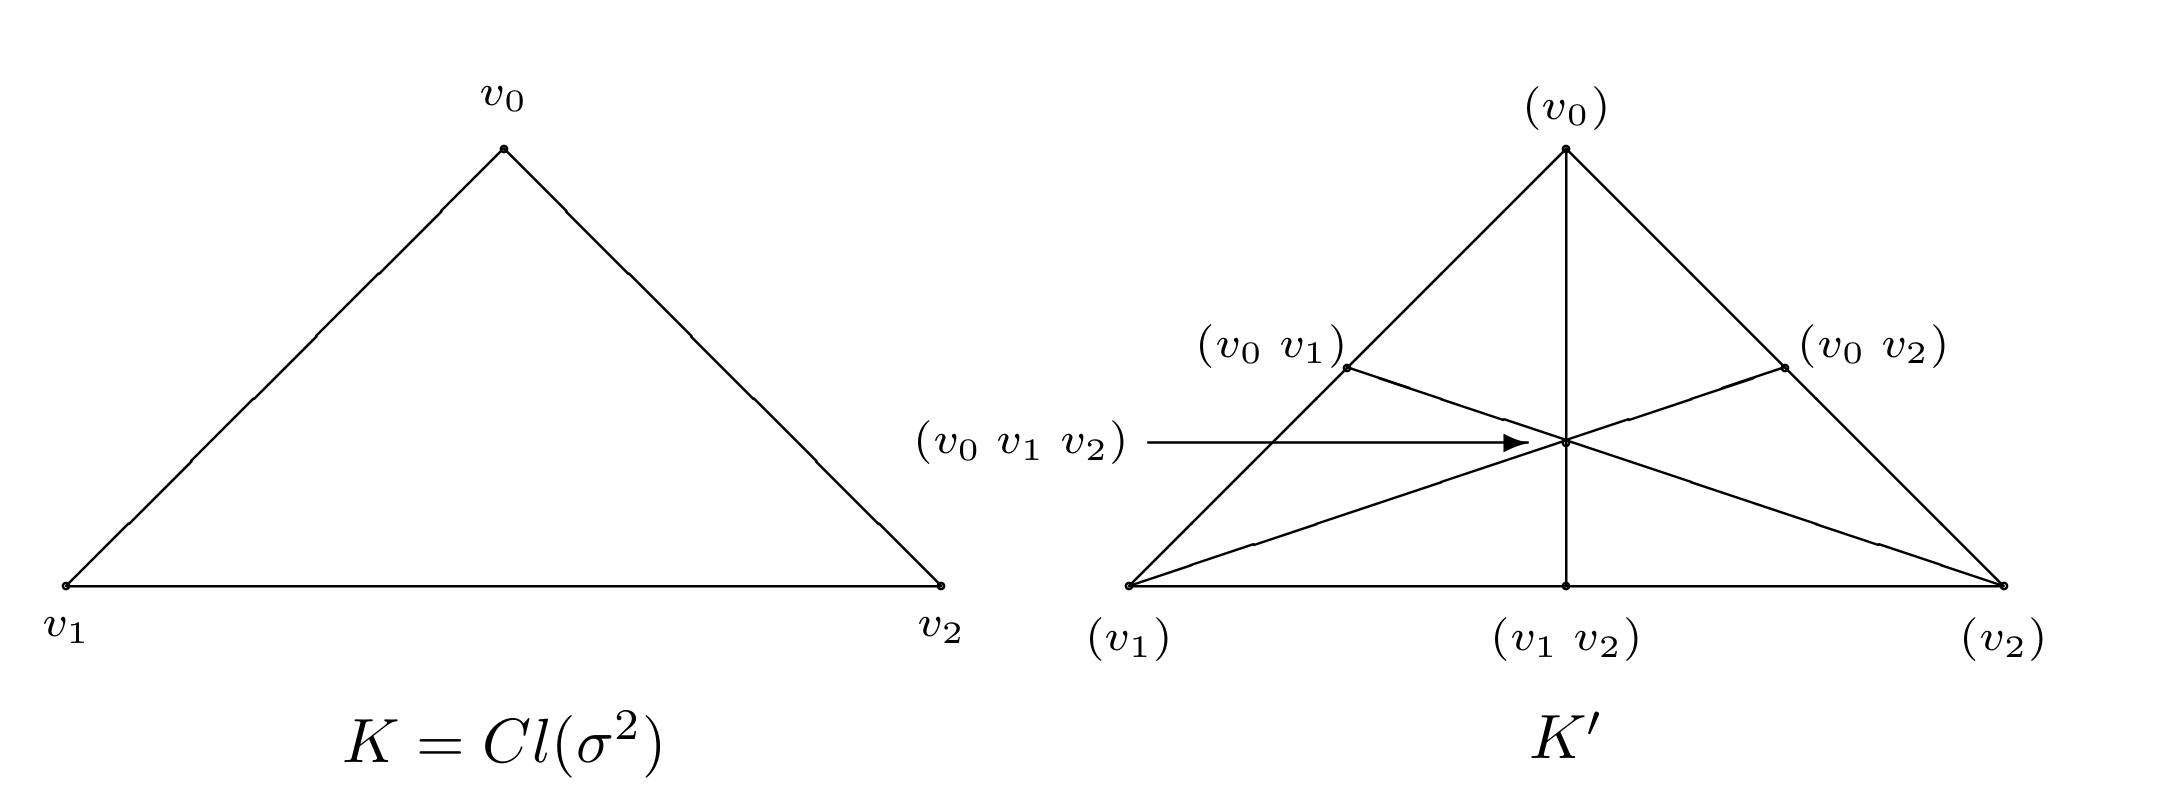
\includegraphics[scale=0.3]{barycentirc subdivision.png}
    \caption{ 重心细分 }
    \label{}
\end{figure}


\begin{definition}
    令 \(  K  \)是单纯复形.定义 \(  K  \)的网径,记作 \(  \mathrm{mesh}\left( K \right)   \),为 \[
    \mathrm{mesh}\left( K \right) =  \max \left\{ \mathrm{diam}\left(  \sigma  \right):  \sigma \text{是}K\text{的一个单形}  \right\} 
    \]   
\end{definition}


\begin{lemma}
    令 \(   \sigma   \)是正维数的单形.则存在 \(   \sigma   \)的顶点 \(  v,w  \),使得   \(  \mathrm{diam}\left(  \sigma  \right)    =  \left\| v-w \right\|\)  .
\end{lemma}

\begin{proof}
    只需要证明同一单形上任意两点的距离都小于等于某两个顶点的距离即可.

    令 \(   \sigma  = \left< v_0,\cdots,v_{q}    \right>   \), \(  x,y \in  \sigma   \).令 \(  y = \sum _{i= 0}^{q}t_{i} v_{i}     \)   .
    则 \[
    \begin{aligned}
    \left\| x-y \right\|  & =  \left\| \sum _{i= 0}^{q}t_{i}x-\sum _{i= 0}^{q}t_{i}v_{i} \right\|\\ 
     & \le \sum _{i= 0}^{q} t_{i} \left\| x- v_{i} \right\|\\ 
      & =\max_{i= 0, 1,\cdots,q }  \left\| x-v_{i} \right\|
    \end{aligned}
    \]对于每个 \(  i= 0, 1,\cdots,q    \),用 \(  v_i \)代替 \(  x  \),用 \(  x  \)代替 \(  y  \),得到 \[
    \left\|v_{i}-x \right\|\le \max _{j= 0, 1,\cdots,q } \left\| v_{j}-v_{i} \right\|
    \]     综合以上两式,我们得到对于任意的 \(  x, y \in  \sigma   \), \[
    \left\| x-y \right\|\le  \max _{i,j= 0, 1,\cdots,q } \left\| v_{j}-v_{i} \right\|
    \] 另一方面,对于任意的 \(  i,j = 0, 1,\cdots,q   \), \(  \left\| v_{j}-v_{i} \right\|  \le \mathrm{diam}\left(  \sigma  \right) \),因此 \[
    \max _{i,j= 0, 1,\cdots,q } \left\| v_{j}-v_{i} \right\| =  \mathrm{diam}\left(  \sigma  \right) 
    \]  特别地,由于 \(  K  \)中只有有限个单形,我们可以令 \(   \sigma   \)是 \(  \mathrm{diam}  \)最大的 \(  K  \)的单形,   
    并取 \(  v,w  \)为 \(   \sigma   \)的距离最大的两个顶点,于是就有 \[
    \left\| v-w \right\|= \mathrm{diam}\left(  \sigma  \right)=  \mathrm{mesh}\left( K \right)  
    \]  

    \hfill $\square$
\end{proof}

\begin{theorem}
    令 \(  K  \)是正维数的单纯复形,则 \(  \lim_{n \to \infty} \mathrm{mesh}\left( K^{\left( n \right) } \right)= 0   \)  
\end{theorem}

\begin{proof}
    设 \(  K  \)是正维数的单纯复形,  \(  \operatorname{dim}\,K= m  \).
    设 \(  K^{\left( n \right) }  \)是 \(  K  \)的第\(  n  \)重心细分.考察 \(  K^{\left( n+ 1 \right) }  \)的网径,由引理知存在 \(  K^{\left( n+ 1 \right) }  \)的两个顶点 \(  \dot{\tau}, \dot{\sigma}  \),使得  \[
    \mathrm{mesh}\left( K^{\left( n+ 1 \right) } \right) =  \left\| \dot{\tau}-  \dot{\sigma} \right\| 
    \]并且 \(  \tau , \sigma   \)是 \(  K^{\left( n \right) }  \)的两个单形,使得\(   \sigma   \)是\(  \tau   \) 的一个面, \(   \dot{\sigma}  \)和 \(  \dot{\tau}  \)分别是对应的重心.         
    设 \(   \tau  =  \left<  v_0,\cdots,v_{q}    \right>   ,q \le m\).则 \(   \dot{\tau}=  \sum _{i= 0}^{q} \frac{1}{q+ 1} v_{i} \),我们有 \[
    \begin{aligned}
    \mathrm{mesh}\left( K^{\left( n+ 1 \right) } \right)  & =  \left\| \dot{\tau}- \dot{\sigma} \right\|\\ 
     & =  \left\| \sum _{i= 0}^{q} \left( \frac{1}{q+ 1}v_{i}- \frac{1}{q+ 1} \dot{\sigma}  \right) \right\|\\ 
      & \le \sum _{i= 0}^{q} \frac{1}{q+ 1}\left\| v_{i}-  \dot{\sigma} \right\|\\ 
       & \le  \frac{q}{q+ 1} \mathrm{mesh}\left( K^{\left( n \right) } \right) \\ 
        & \le  \frac{m}{m+ 1} \mathrm{mesh}\left( K^{\left( n \right) } \right) 
    \end{aligned}
    \]  因此 \[
    0 \le  \lim_{n \to \infty} \mathrm{mesh}\left( K^{\left( n \right) } \right) \le  \mathrm{mesh}\left( K \right) \lim_{n \to \infty}\left( \frac{m}{m+ 1} \right)   ^{n} = 0
    \]
    \hfill $\square$
\end{proof}


\begin{theorem}{单纯估计定理}
    令 \(  f: \left| K \right|\to \left| L \right|    \) 是连续映射.则存在 \(  K  \)的重心细分 \(  K^{\left( k \right) }  \),
    以及单纯映射 \(  g: K^{\left( k \right) } \to L  \),使得 \(  g  \)是 \(  f  \)的一个单纯估计.特别地, \(  \left| g \right|: \left| K^{\left( k \right) }  \right|   = \left| K \right|\to \left| L \right|   \)同伦于 \(  f  \).       
\end{theorem}

\begin{proof}
     \(  \left\{ \mathrm{ost}\left( v \right): v\text{是 } L \text{的一个顶点}  \right\}  \) 构成 \(  \left| L \right|   \)的一个开覆盖,由于 \(  \left| L \right|   \)是紧的度量空间,它存在Lebesgue数 \(  \eta   \),使得 \(  \left| L \right|   \)上 任意半径小于 \(  \eta   \)的开球都含于某个 \(  \mathrm{ost}\left( v_0 \right)   \),其中 \(  v_0  \)是 \(  L  \)的一个顶点   .
     又 \(  \left| K \right|   \)是紧的度量空间, \(  f  \)是连续映射,    因此 \(  f  \)在 \(  \left| K \right|   \)上一致连续,从而存在 \(  \delta >0  \),使得对于任意的 \(  x_1,x_2 \in \left| K \right|   \),只要
      \(  \left\| x_1-x_2 \right\|<  \delta   \),就有 \(  \left\| f\left( x_1 \right)-f\left( x_2 \right)   \right\|< \eta   \).由 \(  \lim_{n \to \infty} \mathrm{mesh}\left( K^{\left( n \right) } \right)= 0   \),可知存在 \(  k \in \mathbb{N}   \),使得
       \(  \mathrm{mesh}\left( K^{\left( k \right) } \right)< \frac{1}{2}  \delta     \).现在,任取 \(  K^{\left( k \right) }  \)的顶点 \(  v  \),则 \(  \mathrm{ost}\left( v \right)   \)含于 \( \left| K \right|   \)上以 \(  v  \)为原点, \(  \frac{1}{2}  \delta    \)为半径的开球,
       进而 \(  f\left( \mathrm{ost}\left( v \right)  \right)   \)含于以 \(  f\left( v \right)   \)为原点, \(  \eta   \)为半径的开球 ,进而存在 \(  \left| L \right|   \)的顶点 \(  v^{\prime}   \),使得 \[
       f\left( \mathrm{ost}\left( v \right)  \right)\subseteq \mathrm{ost}\left( v^{\prime}  \right)  
       \]这表明 \(  K^{\left( k \right) } \)是关于 \(  f  \)星相关于 \(  L  \)的,由星相关情况的单纯估计定理\ref{star-related-Simp-Appro-thm},此定理成立.           
      

    \hfill $\square$
\end{proof}


\begin{definition}{n-连通}
    称拓扑空间 \(  X  \)是 \(  n -1 \)-连通的(\(n\ge 0  \)   ),若对于每个 \(  k\le n  \), 任意从 \(  \mathbb{S}^{k}  \)到 \(  X  \)的连续映射都是零伦.   
\end{definition}

\begin{theorem}
    对于每个 \(  n\ge 1  \), \(  \mathbb{S}^{n}  \)是 \(  \left( n-1 \right)   \)-连通的.   
\end{theorem}

\begin{proof}
    任取 \(  k\le n  \),设 \(   \sigma ^{k+ 1}  \)和 \(   \sigma ^{n+ 1}  \)是单形, \(  K  \), \(  L  \)分别表示对应的 \(  k , n  \)骨架.则 \(  K  \)和 \(  \mathbb{S}^{k}  \)同胚, \(  L  \)和 \(  \mathbb{S}^{n}  \)同胚.
    设 \(  h  \)和 \(  h^{\prime}   \)分别设 \(  K  \)到 \(  \mathbb{S}^{k}  \), \(  L  \)到 \(  \mathbb{S}^{n}  \)的同胚映射,任取 \(  \mathbb{S}^{k}  \)到 \(  \mathbb{S}^{n}  \)的连续映射 \(  f  \),我们有交换图                  
    \[\begin{tikzcd}
	{|K|} && {|L|} \\
	{\mathbb{S}^k} && {\mathbb{S}^n}
	\arrow["{g = h\circ f\circ (h^{\prime})^{-1}}", from=1-1, to=1-3]
	\arrow["h"', from=1-1, to=2-1]
	\arrow["{h^{\prime}}", from=1-3, to=2-3]
	\arrow["f"', from=2-1, to=2-3]
\end{tikzcd}\]
    由同伦对复合映射的保持,我们知道 \(  f  \)是零伦当且仅当 \(  g  \)是零伦. 
    由单纯估计定理,存在 单纯映射 \(  g^{\prime} : K\to L  \),使得 \(  g^{\prime}   \)是 \(  g  \)的一个单纯估计,我们也记 \(  g^{\prime}   \)的诱导映射为 \(  g^{\prime} : \left| K \right|\to \left| L \right|    \),则 \(  g^{\prime}   \)和 \(  g  \)同伦  .     
    注意到从低维单纯复形到高维单纯复形的单纯映射一定是非满的,因此存在 \(  p \in \left| L \right|   \),使得 \(  g^{\prime} : \left| K \right|\to  \left| L \right|-\left\{ p \right\}    \).又 \(  \left| L \right|-\left\{ p \right\}   \)同胚于 \(  \mathbb{S}^{n}\setminus \left\{ h^{\prime} \left( p \right)  \right\}  \),进而通过球极投影同胚于可缩空间 \(  \mathbb{R} ^{n}  \).我们发现 \(  \left| L \right|-\left\{ p \right\}   \)是可缩的,因此 \(  g^{\prime}   \)是零伦,进而 \(  g, f  \)均是零伦.
    这表明 \(  \mathbb{S}^{n}  \)是 \(  \left( k-1 \right)   \)-连通的, 由 \(  k  \)的任意性可知命题成立.           
    \hfill $\square$
\end{proof}




\begin{corollary}
     \(  n  \)-球面 \(  \mathbb{S}^{n}  \), \(  n\ge 2  \)是单连通的.   
\end{corollary}


\section{广义单纯复形}

观察单形和单纯复形的形式,我们可以将顶点抽象成点单集,2-单形抽象成二元集,以此类推, \(  k  \)-单形抽象成 \(  k  \)元素集.
对面的封闭性,就可以看是对元素的非空子集的封闭性,例如若要使 \(  \left\{ \left\{ a,b \right\} \right\}  \)对取子集封闭,需要添加 \(  \left\{ a \right\}  \)和 \(  \left\{ b \right\}  \),得到 集合 \(  \left\{ \left\{ a,b \right\},\left\{ a \right\},\left\{ b \right\} \right\}  \)    .
这样就可以抽象出单纯复形的概念.

对于抽象的单形的实现,可以先看成是顶点的形式和空间的一个系数和为1的子集,再将其对偶地嵌入到欧氏空间当中去.由于我们可以直接将单形嵌入到无穷维实对偶空间上去,
可以放宽单纯复形的条件,允许定义任意由任意多个单形组合在一起,得到广义单纯复形的概念,它的几何对象可以在无穷维欧氏空间上得到实现.

单纯复形的几何实现上可以自然地赋予两种拓扑,一种是相干拓扑,一种是无穷维欧氏空间的子空间拓扑.考虑到将单纯复形视为单形的组合的观点,我们通常赋予几何实现以前者的拓扑. 

\begin{introduction}
    \item 抽象单纯复形
    \item 抽象单纯复形的几何实现
    \item 多面体及其拓扑-相干拓扑
\end{introduction}

\begin{definition}
    一个\textbf{抽象单纯复形}是指有限个非空子集构成的集合 \(  K  \),使得 若 \(  A  \)是 \(  K  \)中的元素,则 \(  A  \)的任意非空子集亦然. 
    
    称 \(  K  \)中的每一个元素为一个单形. 
\end{definition}

\begin{definition}
    设 \(  \mathcal{K}  \)是抽象单纯复形, \(  \left\{ v_{ \alpha }: \alpha  \in J \right\}  \)是  \(  \mathcal{K}  \)   的顶点集,其中 \(  J  \) 是指标集.
    考虑集合 \[
    \mathbb{R}^{J} =  \left\{ f: J\to \mathbb{R} : f\left( v_{\alpha } \right)= 0\text{对于除有限个} \alpha \text{外成立}  \right\}
    \]则显然 \(  \mathbb{R}^{J}  \)是 \(  \mathbb{R}   \)-线性空间,可以分解为 \(  J  \)的基数多个 \(  \mathbb{R}   \)的直和.    
\end{definition}

\begin{remark}
    \begin{enumerate}
        \item  \(  \mathbb{R} ^{J}  \)上有自然的基 \(  \left\{ \varepsilon _{\alpha } : \alpha  \in J\right\}  \), 其中 \[
        \varepsilon _{\alpha }\left( \beta  \right) = \begin{cases} 1,&\beta = \alpha \\ 
         0,& \beta \neq \alpha  \end{cases}  
        \]  
        \item \(  \mathbb{R} ^{J}  \)上可以定义度量 \[
        d\left( f,g \right)=  \sqrt{\sum _{\alpha  \in J} \left( f\left( v_{\alpha } \right)-g\left( v_{ \alpha } \right)   \right)^{2} } 
        \] 
    \end{enumerate}
    
\end{remark}

\begin{definition}{几何实现}
    设 \(  \mathcal{K}  \)是单纯复形, \(  \left( v_{\alpha _0 },\cdots ,v_{\alpha _k } \right)   \)是 \(  \mathcal{K}  \)的一个 \(  k  \)-单形.
    称集合 \[
    \left\{ f \in \mathbb{R} ^{J}: \sum _{0}^{k} f\left( v_{\alpha _i } \right)= 1, 0\le f\left( v_{\alpha _i } \right)\le 1   \right\} =  \left\{ \sum _{0}^{k} t_{i} \varepsilon _{\alpha _i } : \sum _{0}^{k}t_{i}= 1, 0\le t_{i}\le 1\right\}
    \]为 \(  \left( v_{\alpha _0 },v_{\alpha _1 },\cdots ,v_{\alpha _k } \right)   \)对应的几何单形.  \(  \mathcal{K}  \)的全体集合单形的并被称为是 \(  \mathcal{K}  \)的几何实现,记作 \(  \left| K \right|   \).   
\end{definition}

\begin{enumerate}
    \item  \(  \left| K \right|   \)上存在 \(  \mathbb{R} ^{J}  \)的子空间拓扑,并且有继承的度量,对应的拓扑空间记作 \(  \left| K \right|_{d}   \). 
\end{enumerate}

\begin{definition}
    设 \( \mathcal{K}  \) 是抽象单纯复形, \(  \left| K \right|   \)是它的几何实现.
     \(  \left| K \right|   \)的每个几何单形都位于一个有限为欧氏空间上, 在取对应的子空间拓扑下为紧的空间.
    定义 \(  \left| K \right|   \)上的相干拓扑,为使得所有含入映射 \(  i:\left( \varepsilon _{\alpha _0 },\varepsilon _{\alpha _1 },\cdots ,\varepsilon _{\alpha _k } \right)\to \left| K \right|    \)连续的最精细的拓扑,其中 \(  \left( \varepsilon _{\alpha _0 },\cdots ,\varepsilon _{\alpha _k } \right)   \)是 \(  \mathcal{K}  \)的任意几何单形.
    对应的拓扑空间就记作 \(  \left| K \right|   \) ,称为是广义单纯复形或多面体.换言之, \(  F  \)是 \(  \left| K \right|   \)上的开集,当且仅当对于任意的 \(  \left| K \right|   \)的几何单形 \(   \sigma   \), \(  F\cap  \sigma   \)     是闭集.
\end{definition}

\begin{definition}
    称拓扑空间 \(  X  \)是可三角剖分的,若存在抽象单纯复形 \(  K  \),以及同胚映射 \(  f: \left| K \right|\to X   \),其中 \(  \left| K \right|   \)被赋予相干拓扑.    
\end{definition}


\begin{theorem}
    令 \(  X  \)是拓扑空间, \(  f: \left| K \right|\to X   \)是映射.则 \(  f  \)连续当且仅当对于每个 \(  K  \)的单形 \(   \sigma   \), \(  f|_{ \sigma }  \)连续.      
\end{theorem}

\begin{proof}
    连续映射的限制映射也是连续的,只需要证明反方向.

    若对于任意的单形 \(   \sigma \in K  \), \(  f|_{ \sigma }  \)连续,令 \(  F  \)是 \(  X  \)的闭集,则对于每个 \(   \sigma   \), \[
    \left( f|_{ \sigma } \right)^{-1}  \left( F \right) =  f^{-1} \left( F \right)\cap  \sigma    
    \]     是 \(   \sigma   \)上的闭集,因此 \(  f^{-1} \left( F \right)   \)在 \(  \left| K \right|   \)上是闭的.这表明 \(  f  \)连续.    

    \hfill $\square$
\end{proof}

\begin{proposition}
    令 \(  L  \)是 \(  K  \)的子单形,则 \(  \left| L \right|   \)是 \(  \left| K \right|   \)的闭子空间.    
\end{proposition}

\begin{theorem}
    多面体 \(  \left| K \right|   \)是Hausdorff的. 
\end{theorem}



\begin{problemset}
    \item 令 \(   \sigma ^{n} =  \left< v_0,\cdots,v_{n}    \right>  \)是 \(  n  \)-单形,给出 \(   \sigma ^{n}  \)的面数的公式.   
    \begin{proof}
        面数即为 \(  \mathrm{Cl}\left(  \sigma  \right)   \)的元素个数一一对应,而 \(  \mathrm{Cl}\left(  \sigma  \right)   \)与 \(  \left\{  a_0,\cdots,a_{n}    \right\}  \)的全体非空子集一一对应,个数为 \(  2^{n}-1  \).    
    
        \hfill $\square$
    \end{proof}

     \item 证明 \(  \mathbb{R} ^{n}  \) 的每个紧 的凸子集都是可三角剖分的.
    \begin{proof}
       
        \(  \mathbb{R} ^{n}  \)上的紧凸子集是否是流形? 
    
        \hfill $\square$
    \end{proof}
\end{problemset}

\end{document}